\documentclass{article}
\usepackage[utf8]{inputenc}
\usepackage[T1]{fontenc}
\usepackage{natbib}
\usepackage{hyperref}
\usepackage{graphicx} % Required for inserting images
\usepackage{listings}
\usepackage{xcolor}
\usepackage{amsmath}
\usepackage{algorithm}
\usepackage{algorithmic}
\usepackage{algpseudocode}

\lstset{
    backgroundcolor=\color{lightgray}, % background color
    basicstyle=\footnotesize\ttfamily, % font size and type
    breaklines=true, % enables line breaking
    frame=single, % adds a frame around the code
    numbers=none, % disable line numbers
    keywordstyle=\color{blue}, % keyword color
    commentstyle=\color{green}, % comment color
    stringstyle=\color{red}, % string color
    linewidth=1.2\textwidth, % adjusts the width of the code block
    xleftmargin=-6em, % left margin for the code block
    xrightmargin=-1em % right margin for the code block
}

\lstset{language=C++,
    morekeywords={__syncthreads, uint16_t, threadIdx}, % Add CUDA-specific keywords
    commentstyle=\color{green!50!black}, % Adjust comment color
    basicstyle=\footnotesize\ttfamily
}

\title{PMPH group project: Sorting on GPUs}
\author{Mathias Heldbo (tzc182), Rasmus Gabelgaard Nielsen (ncg106) \\ and Hans Peter Lyngsøe (pvr448)}
\date{November 2024}

\begin{document}

\maketitle

\section{The radix sort algorithm }
Radix sort is a very important and efficient sorting algorithm, in this section we will discuss the sequential implementation as well as parallelization using basic blocks.
\begin{itemize}
\item Radix sort: \\
The basic idea of radix sort is to sort an integer into digits of the form $2^r$ consisting of r bits. Then the list is sorted for each digit until all digits have been traversed and the list is fully sorted. The main assumptions of radix sort is that all integers in the input list are of fixed length, and can all be represented as bits, that the integer or string can be split into digits/keys with a known and limited range, and that we have a stable sorting algorithm for each digit, such as counting sort. 
\item Radix sort sequential: \\
The sequential implementation iterates through the digits, r bits at a time. The simplest implementation does 1 bit at a time, but larger r can improve locality. Each digit m, has r bits, such that $m = 2^r$. Radix sort works by performing a counting sort or other stable sort on each set of digits, until all digits have been traversed. Counting sort follows the following syntax: 
\begin{figure} [H]
    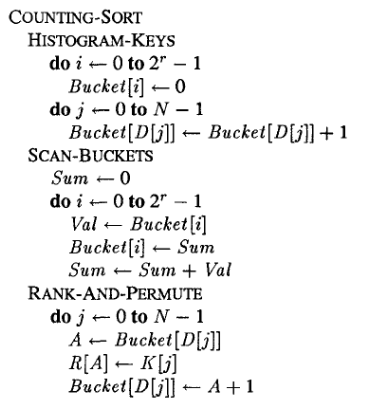
\includegraphics[width=0.5\linewidth]{images/count_sort.PNG}
    \caption{Counting Sort \citep{zagharadixvector}}
    \label{fig:enter-label}
\end{figure}.

Where Histogram-Keys counts the number of elements in a bucket for each unique digit. Scan-Buckets, scan the buckets and returns the position at which the first element of a subset having a certain digit is to be placed, that is, the offset. Finally, Rank-and-permute matches the digit value with the bucket offset and iterates through each "sub bucket" to order the elements by their digit. After this, counting sort, or another sort, is repeated on each subset of digits until the whole list is sorted.

\item For parallelization of radix sort, similar ideas are used, however, there are a few key differences. One such method is discussed in \citep{zagharadixvector}. With p processors, the input list is split into p sub-lists for each processor to work on. Each processor performs Histogram-keys locally to create local histograms, then a global scan is performed across buckets to calculate the global offset, Rank and Permute can then be performed locally and written to global memory as Rank and Permute takes in the offset, and therefore there are no dependencies across processors \citep{zagharadixvector}. 

Let us now consider a very simple parallel radix sort implementation going through 1 bit at a time, for 32- bit integers using basic blocks, and let us consider the example of
$$\begin{bmatrix} 1, 4, 2, 3\end{bmatrix}$$
with a bit representation of: 
$$\begin{bmatrix} 001, 100, 010, 011\end{bmatrix}$$
Please bear in mind that this implementation is a very simplified parallel radix sort implementation in Futhark using basic blocks such as map, scan, reduce and scatter. Due to its syntax, Futhark automatically distributes the processes depending on available processors, however, better approaches are discussed in part 2. 
\begin{lstlisting}
-- xs = [1,4,2,3] in integer format
-- xs = [001, 100, 010, 011] in bit format 
def radix_bit [n] `t (f: t -> u32) (arr: [n]t) (b: i32): [n]t =
(1)    let bits = map(\x -> (i32.u32 (f x >> u32.i32 b )) & 1) xs -- [1, 0, 0, 1]
                                                                  -- D = O(1), W = O(n)
(2)    let bits_neg = map (1-) bits                               -- [0, 1, 1, 0]
                                                                  -- D = O(1), W = O(n)
(3)    let offs = reduce (+) 0 bits_neg                           -- 2, 
                                                                  -- D = O(log n), W = O(n)
(4)    let idxs0 = map2 (*) bits_neg (scan (+) 0 bits_neg)        -- [0, 1, 2, 0],
                                                                  -- D = O(log n), W = O(n)
(5)    let idxs1 = map2 (*) bits (map (+offs) (scan (+) 0 bits))  -- [3, 0, 0, 4], 
                                                                  -- D = O(log n), W = O(n)
(6)    let idxs2 = map2 (+) idxs0 idxs1                           -- [3, 1, 2, 4]
                                                                  -- D = O(1), W = O(n)
(7)    let idxs = map (\x -> x-1) idxs2                           -- [2, 0, 1, 3]
                                                                  -- D = O(1), W = O(n)
(8)    let xs` = scatter (copy xs) idxs xs                        -- [4, 2, 1, 3]
                                                                  -- D = O(1), W = O(n)
        -- in terms of the bit in question, it becomes [100, 010, 001, 011]
(9)    in xs`                                                                                                                                -- D = O(log n), W = O(n)

def radix [n] `t (f: t -> u32) (xs: [n]t): [n]t = 
(10)    loop xs for i < 32 do radix_bit f xs i                     -- D = O(log n), W = O(n)
\end{lstlisting}

This implementation is from \href{https://futhark-lang.org/examples/radix-sort-key.html}{radix-sort-key (futhark-lang.org)}, and applied to each bit of 32 bit unsigned integers, as radix sort requires each digit to be in the range of 0 to m-1. The radix\_bit part of the algorithm takes in a bit. The bits are stored in bits (1), bits\_neg (2) contains the bits converted to their compliment, offs (3), get the offsets of the bits by calculating how many 0 bits there are, which is what bits\_neg is used for. Offs is similar to what histogram keys does, when considering a digit of size 2, as in this case. Idxs0 (4) finds the indices of elements with a bit of 0, while idxs1 (5) finds the indices of elements with a bit of 1, and idxs2 (6) concatenate those two lists. Indexes are then stored in idxs (7) assuming zero indexing, by subtracting 1 from every index. The idxs calculation contains the scan part of the algorithm. Then scatter (8) is used to distribute the elements to their corresponding location, like rank and permute would, but it does the operations in a slightly different way, while keeping the overall structure of radix sort and its syntax intact. 
\\ \\
Let us now consider the work depth complexity, for a list of length n, the work and depth complexity is written next to the code, where scan and reduce both have a depth complexity of O(log n), and all lines have O(n) work complexity, as they traverse n elements. While this work depth complexity might seem good on paper, this is a best case scenario, in which we always have n processors. More advanced methods deal with the distribution of the workload in a fashion more suited to the GPU, and this improves the overall speed and efficiency of the algorithm. 
\end{itemize}

\section{Fast parallel radix sort}

Although \citep{zagharadixvector} was great at the time, our literature search provided several higher performing parallel radix sorts. The first implementation by Satish et. al. provides a significant speed up from previous methods using the following ground principles.
\begin{figure} [H]
    \centering
    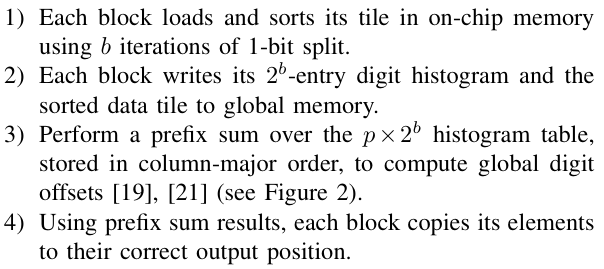
\includegraphics[width=\linewidth]{report/images/satish.PNG}
    \caption{Satish steps \citep{satish}}
    \label{fig:enter-label}
\end{figure} Furthermore, parallel local radix counting and pre-sorting as well as global radix ranking and coalesced global shuffling was also done by \citep{satish}. Building off these concepts, Ha. et. al proposed two improvements, implicit counting and a mixed-data structure with 4 elements, that is 2-bit digits.
\begin{itemize}
\item Implicit counting \\
Uses bit shifting to create a 32-bit register for radix value 0, 1 and 2. With the count of 0 assigned to bits from 0 to 9, the count of 1 assigned to bit values from 10-19, and the count of 2 assigned to bits from 20-29. The implicit count is: $$impl_{cnt} = cnt_0 + (cnt_1 \ll 10) + (cnt_2 \ll 20)$$
The implicit value is: 
$$impl_{val} = (val \lt  3) \ll (10 \cdot val)$$
$impl_{cnt}$ is calculated by incrementing by the $impl_{val}$:
$$impl_{cnt} = impl_{cnt} + impl_{val}$$
The count is retrieved by: 
$$cnt\begin{bmatrix}val\end{bmatrix} = impl_{cnt} \gg (10 \cdot val) $$
and the fourth counting value is retrieved by:
$$cnt\begin{bmatrix} 3 \end{bmatrix} = idx - cnt\begin{bmatrix} 0 \end{bmatrix} - cnt\begin{bmatrix} 1 \end{bmatrix} - cnt\begin{bmatrix} 2 \end{bmatrix}$$
Thus implicit counting reduces the count operations from 4 in Satish. et. al to 2. 
\item Mixed-data structure \\

\begin{figure} [H]
    \centering
    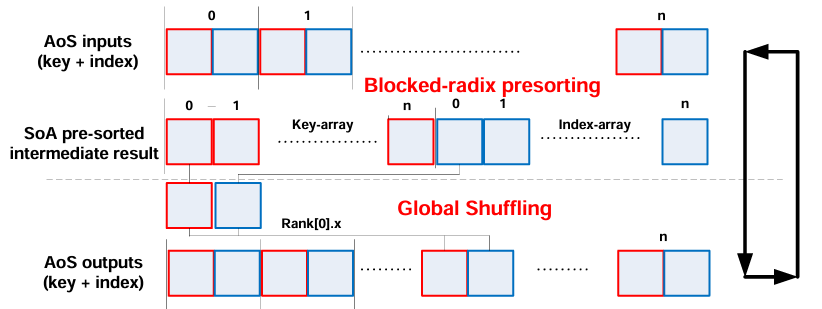
\includegraphics[width=\linewidth]{images/mixed-data.PNG}
    \caption{Mixed data method \citep{ha2010implicit}}
    \label{fig:enter-label}
\end{figure}
Ha. et. al's hybrid data structure uses AoS and SoA, which reduces suboptimal coalesced scattering effects, and requires only one shuffle pass on the pre sorting data due to the structure  
\\
We have decided to attempt to implement the Ha. et. al algorithm
\item Pseudocode



\end{itemize}
\begin{lstlisting}
1. Initialize data structures:
   - Load input keys and values.
     * Work: O(n), Depth: O(1)
   - Assuming the input is integers we can map from 32 to 24 bit by:
   - Determine [a,b] using reduce
     * Work: O(n), Depth: O(log n)
   - Map input values from a, b to [0, b-a]
     * Work: O(n), Depth: O(1)
     
2. Iterate through bit shifts:
   For each bit shift (e.g., 4 bits per pass):
     - Map the current bit shift to all elements.
       * Work: O(n), Depth: O(1)
     - Create an array of structures `AoS` by associating each element`s index and key.
       * Work: O(n), Depth: O(1)

3. Local counting and presorting (within each block):
   - For each block of block size B * 4 elements:
     - Compute implicit counts:
       * Work: O(B*4)  per block, total O(n), Depth: O(log B*4)

     - Calculate the local rank for each element in the block using **exclusive scan** on the histogram:
       * Work: O(B*4) per block, total O(n), Depth: O(log B*4)

     - Scatter locally (pre sort):
       * Work: O(B) per block, total O(n), Depth: O(1)

4. Global ranking and offset calculation:
   - Compute global offsets using **prefix sum** (scan) across all local histograms:
     * Work: O(P) = O(n/(B))
     * Depth: O(log P) = O(log n/(B))

   - Adjust local ranks by adding block offsets:
     * Work: O(n), Depth: O(1)

5. Global shuffling and final scatter:
   - Scatter elements globally using computed global offsets:
     * Work: O(n), Depth: O(log B)

6. Repeat until all bits are processed.
   - Number of passes depends on bit width (e.g., for 24-bit keys (mapping from 32 to 24) with 2 bits (4 elements) per pass, we need 16 passes).
   - Total:
     * Work: O(n * #passes), Depth: O(#passes * (log B + log P) = O(#passes * (log B + log (n/B)))
\end{lstlisting}


Additionally, the algorithm has bank conflict-free access, and stores in different arrays to avoid concurrent access. It also does 
mapping of integers from [a,b to 0, b-a], and of floats by mapping from [a,b] to [0.5, 1] to change from 32 bit to 24 bit, giving a 30\% performance increase. It is an approximation, however, it is precise enough for the implementation. Following the work depth complexity, it is virtually the same for both implementations, however, as stipulated before, the sequential approach is unable to utilize the parallel blocks and will therefore be a lot slower. 

Finally, we expect the algorithm to be well suited for the gpu single instruction multiple data model(SIMT) as the algorithm which in its essence is a composition of histogram->scan->scatter maps naturally to the GPU's execution model as these exhibit regular access patterns, avoiding the irregular uncoalesced  access patterns and thread divergence typical of comparison-based sorts. 

\citep{ha2010implicit} 

\section{In depth cuda implementation}

We implement the algorithm by \citep{ha2010implicit} with some minor modifications. We process 8 bits at a time like nvidia´s cub implementation. 

Radix sort can viewed as a sequential application of counting sort across different bit intervals, each iteration maintaining the invariant that the array is sorted with respect to the last bit.

We can break countsort into 4 fundamental kernels.

\begin{itemize}
    \item Histogram kernel
    \item Transpose kernel
    \item Scan kernel
    \item A final rank and permute kernel
\end{itemize}

We follow the possible good values recommended, thus $Q = 22, lgH = 8, H = 256, B = 256$.

\subsection{Histogram kernel}
The parallel cuda-implementation of the histogram processes $Q$ elements per thread. 
We decided to use shared memory while processing the histogram, as otherwise we would have to access global memory many times, which is slower than first using shared memory, and then writing the final histogram to global memory.
Unfortunately we have to use atomic adds for incrementing our histogram buckets which hampers performance due to contention problems as our histograms have few keys. This is done $Q$ times per thread, which is not ideal, as atomic adds impacts performance negatively, which likely affects our results as seen in the last section.
Notably for the histogram we sort each element based on each bit, instead of the regular approach of sorting by each digit. This approach is both more memory efficient and faster.

\subsection{Transpose kernel}

As part of the position computation across buckets we need to compute and update of the ith block and jth key as:
\[
Buckets[i,j]_{after} = \sum_{k=0}^{p-1} \sum_{m=0}^{j-1} Buckets[k,m] + \sum_{k=0}^{i-1} Buckets[k,j]
\]

doing this naively would lead to uncoalesced access as buckets[i, j] and buckets[i+1, j] will be H apart in memory. As we store our matrix in row-major order. In order to efficiently and in a coalesced manner scan our histograms(one for each block) we transpose our matrix such that buckets[i, j] and buckets[i+1, j] will now only be one element apart.
The transpose kernel is relatively simple and is heavily inspired by the one presented in the week 2 assignment. 
We read coalesced from global memory to shared memory(at miniscule performance cost) then read uncoalesced in shared memory and write back coalesced to global memory. As per Cosmin's slides, we use this transpose kernel twice, once before scanning and then again after scanning.
\begin{figure}
  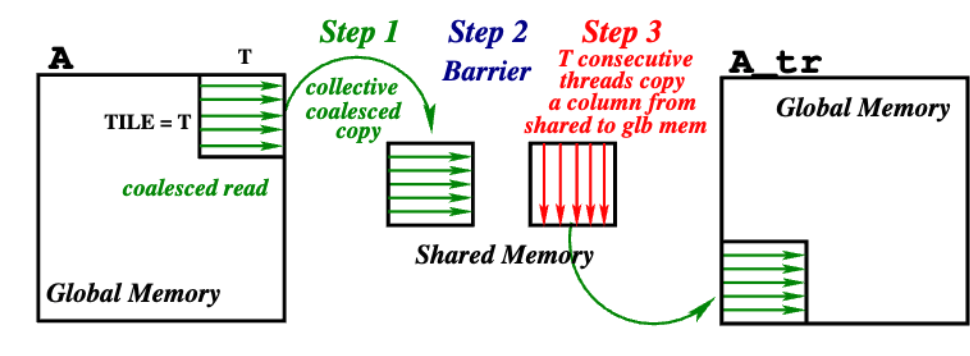
\includegraphics[width=1\textwidth]{images/coalesced_transpose.png}
  \caption{slides/L6-locality.pdf}
\end{figure}


\subsection{Scan kernel}
The scan kernel is called on the transposed matrix to compute the indices for the rank-and-permute kernel. 
We use inclusive scan that performs scan at both the block and warp level, at both levels exploiting the fact that the work depth of scan over an associate binary operator(+) is log(n). We use the efficient implementation of block and warp level scan from assignment2.

\subsection{Rank-and-permute kernel}

This kernel is the most complex and requires deliberate usage of the memory hiearchy to run efficiently on gpus.
First each blocks loads Q*BLOCK\_SIZE elements into shared memory, from there each thread loads its elements from shared memory into its registers.

Next we compute the two-way-partioning sequentially over lgh bits. 
Each thread computes a sequential reduction over its Q elements checking if the i'th bit of a value is set or unset and stores this in shared memory. 
next compute an inclusive scan at the block level computing the cumulative sum of unset bits. 

Each thread then reads from shared memory back to local memory the cumulative sum at their index. 
In this way each thread obtains the necessary information for correctly ordering its elements in shared memory. 
At last each thread reads its new elements from shared back to local memory. And this process is repeated lgH times.

After the two-way partitioning each thread writes its q elements to shared memory and then each block writes its QB elements from shared to global memory. 
Note that we do not have to perform any inter-block communication as all position information has been communicated via the scan across blocks.
We include the inner loop over lgh, the most interessting aspects of the kernel below.

In terms of basic blocks of parallel programming, the rank and permute kernel corresponds to doing a scan/prefix sum and then scattering those elements. 
\newpage

\begin{lstlisting}[language=c++]
  // Sequentially reduce Q elements
        uint16_t accum = 0;
        for (int q_idx = 0; q_idx < P::Q; q_idx++) {
            // we shift by bit to get the bit value and we mask it with 1 to get the boolean value
            // we first shift by the bit_offs offset and then by the current bit from 0 to lgH-1
            uint16_t res = isBitUnset<uint>(bit_offs + bit, reg[q_idx]);
            accum += res;
        }
        
        // the thread local count is stored to shared memory
        local_histo[tid] = accum;

        // we compute the inclusive scan across shared memory
        // to get the cumulative sum of unset bits up to our threadIdx
        uint16_t res = scanIncBlock<Add<uint16_t>>(local_histo, tid);
        __syncthreads();
        local_histo[tid] = res;
        __syncthreads();

        // we get the prefix sum for the entire block
        // which is the cumulative sum of unset bits up to the last thread in the block
        int16_t prefix_sum = local_histo[P::BLOCK_SIZE-1];

        // each thread loads to its registers from shared memory
        // the prefix sum of the previous thread
        if (tid == 0) {
            accum = 0; 
        } else {
            accum = local_histo[tid-1];
        }
        __syncthreads();


        // each thread sequentially rearranges its Q elements
        // and write them to their new position in shared memory
        for (int q_idx = 0; q_idx < P::Q; q_idx++) {
            uint val = reg[q_idx];
            uint16_t bit_val = (uint16_t) isBitUnset<uint>(bit_offs + bit, val);
            
            accum += bit_val;

            int newpos;

            if (bit_val == uint(1)) {
                newpos = accum -1 ;
            } else {
                // we add the prefix of the thread to the local histogram position
                // and we subtract the accumumulator to get the new position
                // we offset by threadIdx.x*Q 
                newpos = prefix_sum + thread_offset + q_idx - accum;
            }
            // we write the element to the new position
            shmem[newpos] = val;
        }
        // wait for all threads to have written their elements
        __syncthreads();


        // each thread loads its new elements from shared memory to its registers
        if (bit < P::lgH-1) {
            // if we are not at the last bit
            // in the new position
            for (int q_idx = 0; q_idx < P::Q; q_idx++) {
                reg[q_idx] = shmem[thread_offset + q_idx];
            }
        } else {
            // if we are at the last bit
            for (int q_idx = 0; q_idx < P::Q; q_idx++) {
                // we iterate with a stride of BLOCK_SIZE
                // but this is not a big deal as uncoalesced 
                // access in shared memory does not affect performance
                uint local_pos = q_idx*P::BLOCK_SIZE + tid;
                reg[q_idx] = shmem[local_pos];
            }
        }
        __syncthreads();
\end{lstlisting}


\subsection{Sorting the whole array}


In order to sort the entire array we apply counting sort in a loop. 
This means our sorting algorithm first takes in a completely unsorted array, then applies all the kernels to it. 
After the rank-and-permute kernel, we overwrite the input array we gave to the histogram and build a new array on the result of the rank-and-permute kernel. 
This process is then repeated, where the histogram is built on the rank-and-permute output, for however many bits our elements in our array have. 
Using 32 bit integers would mean that we launched the kernels 32 times to obtain a fully sorted array. 
Consequently, this can have an effect on the performance of our sorting, \cite{satish}  and \cite{ha2010implicit} suggest that instead of building a histogram for each bit, it is more beneficial to process 4 bits at a time, which leads to only launching the kernels 8 times for 32 bit integers without mapping as explained in part 2. Which is what we do. 
At each iteration except for the last one, we swap our input and output buffer.
While radix-sort does allow for stable sort in a sequential version, our parallel implementation very much depends on which thread accesses memory first for equal elements, thus it is not stable. Consequently, it is not deterministic either. 

\section{Performance evaluation}
We benchmarked cuda, futhark and our own implementation for data types u8, u16, u32, u64.
We use GB/S (gigabytes per second) as our primary performance metric rather than operations per second. This choice is deliberate because radix sort exhibits low arithmetic intensity \citep{ha2010implicit}, making it fundamentally memory-bound rather than compute-bound. GB/S also allows for a good comparison of speed and scalability between the methods.

\begin{figure}[h]
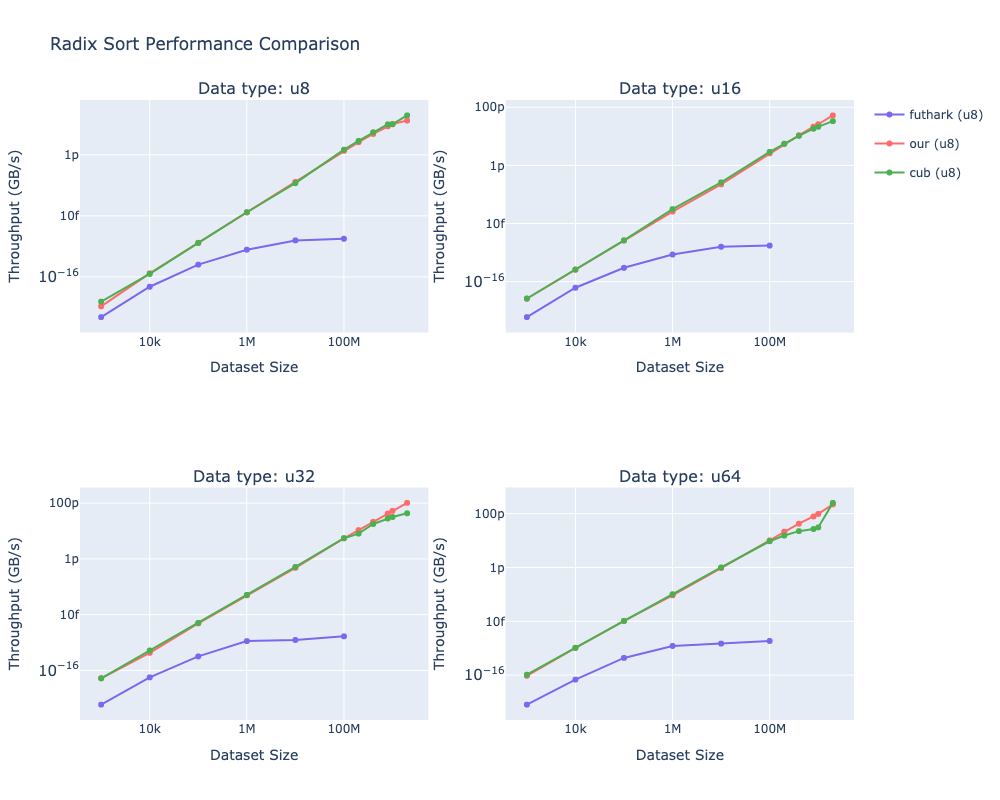
\includegraphics[width=1\textwidth]{images/combined_benchmarks.png}
\end{figure}

Given more time, we would have liked to also benchmark the performance for a fixed array size as a function of key entropy.
Another thing that would be interesting to study is the impact of lgH on our performance, on the one hand increasing lgh would lead to fewer steps of countsort(which would have to be performed sequentially to maintain the invariant)


\subsection{Discussion of results}
The results show that our implementation is comparable to cub's implementation, and is definitely better than the futhark baseline, which was the goal of this project. Notably, we see our implementation performs slightly better than CUB's for uint32\_t keys with large datasets (100M+ keys). This is quite impressive, however it could be possible that the default parameters for CUB could be optimized to yield better results, as we did not find a way to configure the $Q$ or $H$ parameter in CUB. 

\subsection{Suggestions for improving our radix-sort implementation}
As alluded to earlier, we could have processed more bits for our histogram, which could have lead to us launching our kernels fewer times, thus increasing performance. Otherwise there might be some optimizations like decreasing the stride for memory access to global memory in some cases. There is also the possibility that we had one or two too many syncthreads, as we did not have time to properly remove any unnecessary ones. One of the largest performance hits is probably the fact that we use atomic adds. Those can be very slow and while it might be necessary, it could be interesting if we had time to explore methods to avoids those adds, for instance by applying privatization.

\subsection{Usage}


There are multiple options in our makefile. If you want to run both test and measure throughput for our kernel run:
\begin{lstlisting}
make
\end{lstlisting}
from the src folder.

If you wish to test that CUB and our implementation of radix sort runs and validates, please run
\begin{lstlisting}
make test
\end{lstlisting}

If you wish to benchmark all implementations (futhark, cub and ours), run 
\begin{lstlisting}
bash bench_all.bash
\end{lstlisting}

Which will be saved to csv and can be visualized with visualize.ipynb.
Finally if you want to measure throughput for one configuration of either CUB or our implementation run:
\begin{lstlisting}
make run_gpu
./gpu <datatype: u64, u32, u16 or u8> <sizeofarray> <cuda: 0, ours: 1> <maxvalue for datatype>
\end{lstlisting}
Please note, choosing a too small array size might be formatted out while printing and be reported as 0.00 because the throughput is too small. For instance try ./gpu u32 1000000 1 4294967295



\bibliographystyle{plainnat}
\bibliography{references}

\end{document}
